%\documentclass[uplatex,dvipdfmx]{jsarticle}

%\usepackage[dvipdfmx]{graphicx}
%\usepackage{graphicx}
%\usepackage{mathtools}
%\usepackage{cancel}
%\usepackage{amsmath,amssymb}
%\usepackage{cases}
%\usepackage{bm}

%\usepackage{here}
%\usepackage{colortbl}
%\usepackage{feynmf}

%\newcommand{\Slash}[1]{{\ooalign{\hfil/\hfil\crcr\(#1\)}}}

%\begin{document}

%\newpage
%\section{実験}
% -------キリトリ線(上)--------
\subsection{寿命測定のための銅板標的}
寿命測定に用いた銅板標的を図\ref{tar_cu}に示す.
これは厚さ$0.6(\mathrm{mm})\times$横$280(\mathrm{mm})\times$縦$120(\mathrm{mm})$の銅板を木枠に固定したものである.
銅板の縦横の大きさはビームプロファイルから計算されるビームの広がりの約$3\sigma$を止めれるように決めた.
厚さは$4(\mathrm{MeV})$ミューオンが銅板の中心付近で止まるようなものを選んだ.
\subsection{$g$因子測定のための磁場装置}
$g$因子測定に用いた磁場印加標的を図\ref{tar_mag}に記す.
厚さ$0.6(\mathrm{mm})\times$横$80(\mathrm{mm})\times$縦$60(\mathrm{mm})$の銅板を,呼び径$200(\mathrm{mm})$の塩化ビニルパイプの中心にくるように紐で吊るした.
銅板の縦横の大きさはミューオンビームの広がりに対して約$1\sigma$の大きさになるように決めた.
磁石にはセラミック磁石(Y25)を用いており,磁石一束あたりの大きさは厚さ$9(\mathrm{mm})\times$横$10(\mathrm{mm})\times$縦$60(\mathrm{mm})$である.
磁石はパイプの内側に接着剤で貼り付けたうえで,テープで補強した.

\begin{figure}[H]
  \begin{minipage}{0.45\hsize}
    \begin{center}
      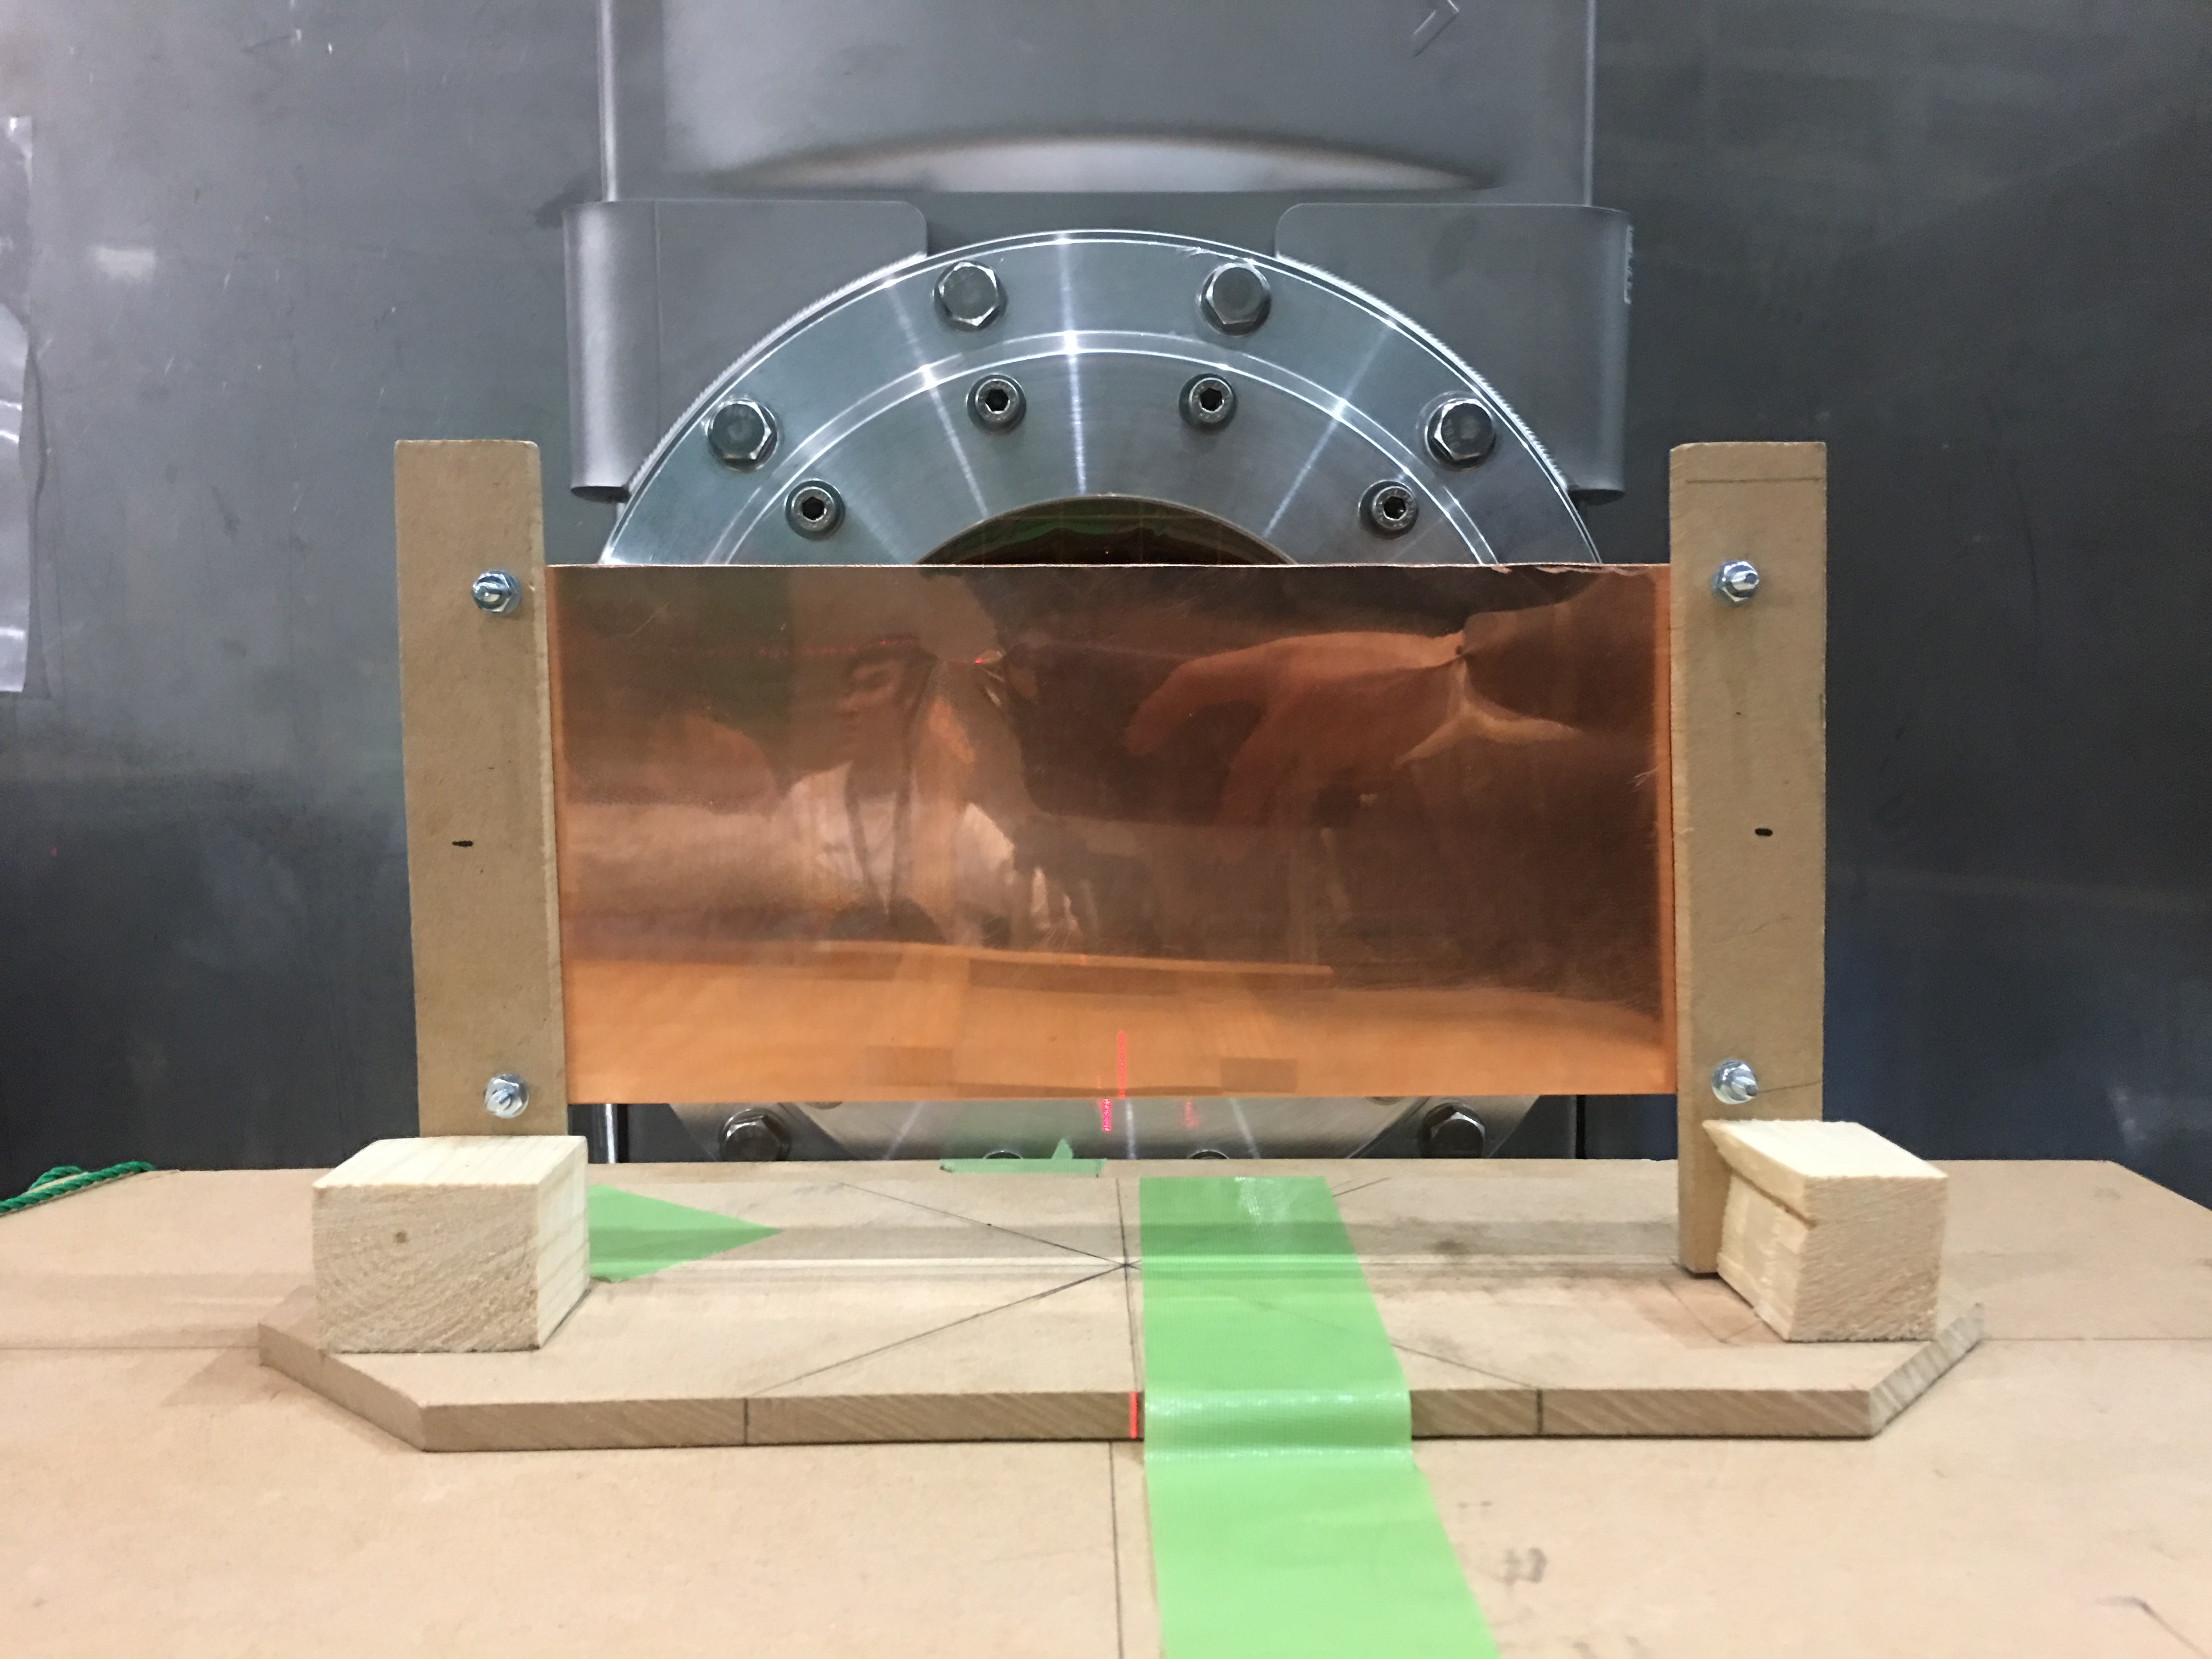
\includegraphics[width=1\textwidth]{figure/tajima/cu_target.jpg}
      \caption{銅板標的}
      \label{tar_cu}
    \end{center}
  \end{minipage}
  \hfill
  \begin{minipage}{0.45\hsize}
    \begin{center}
      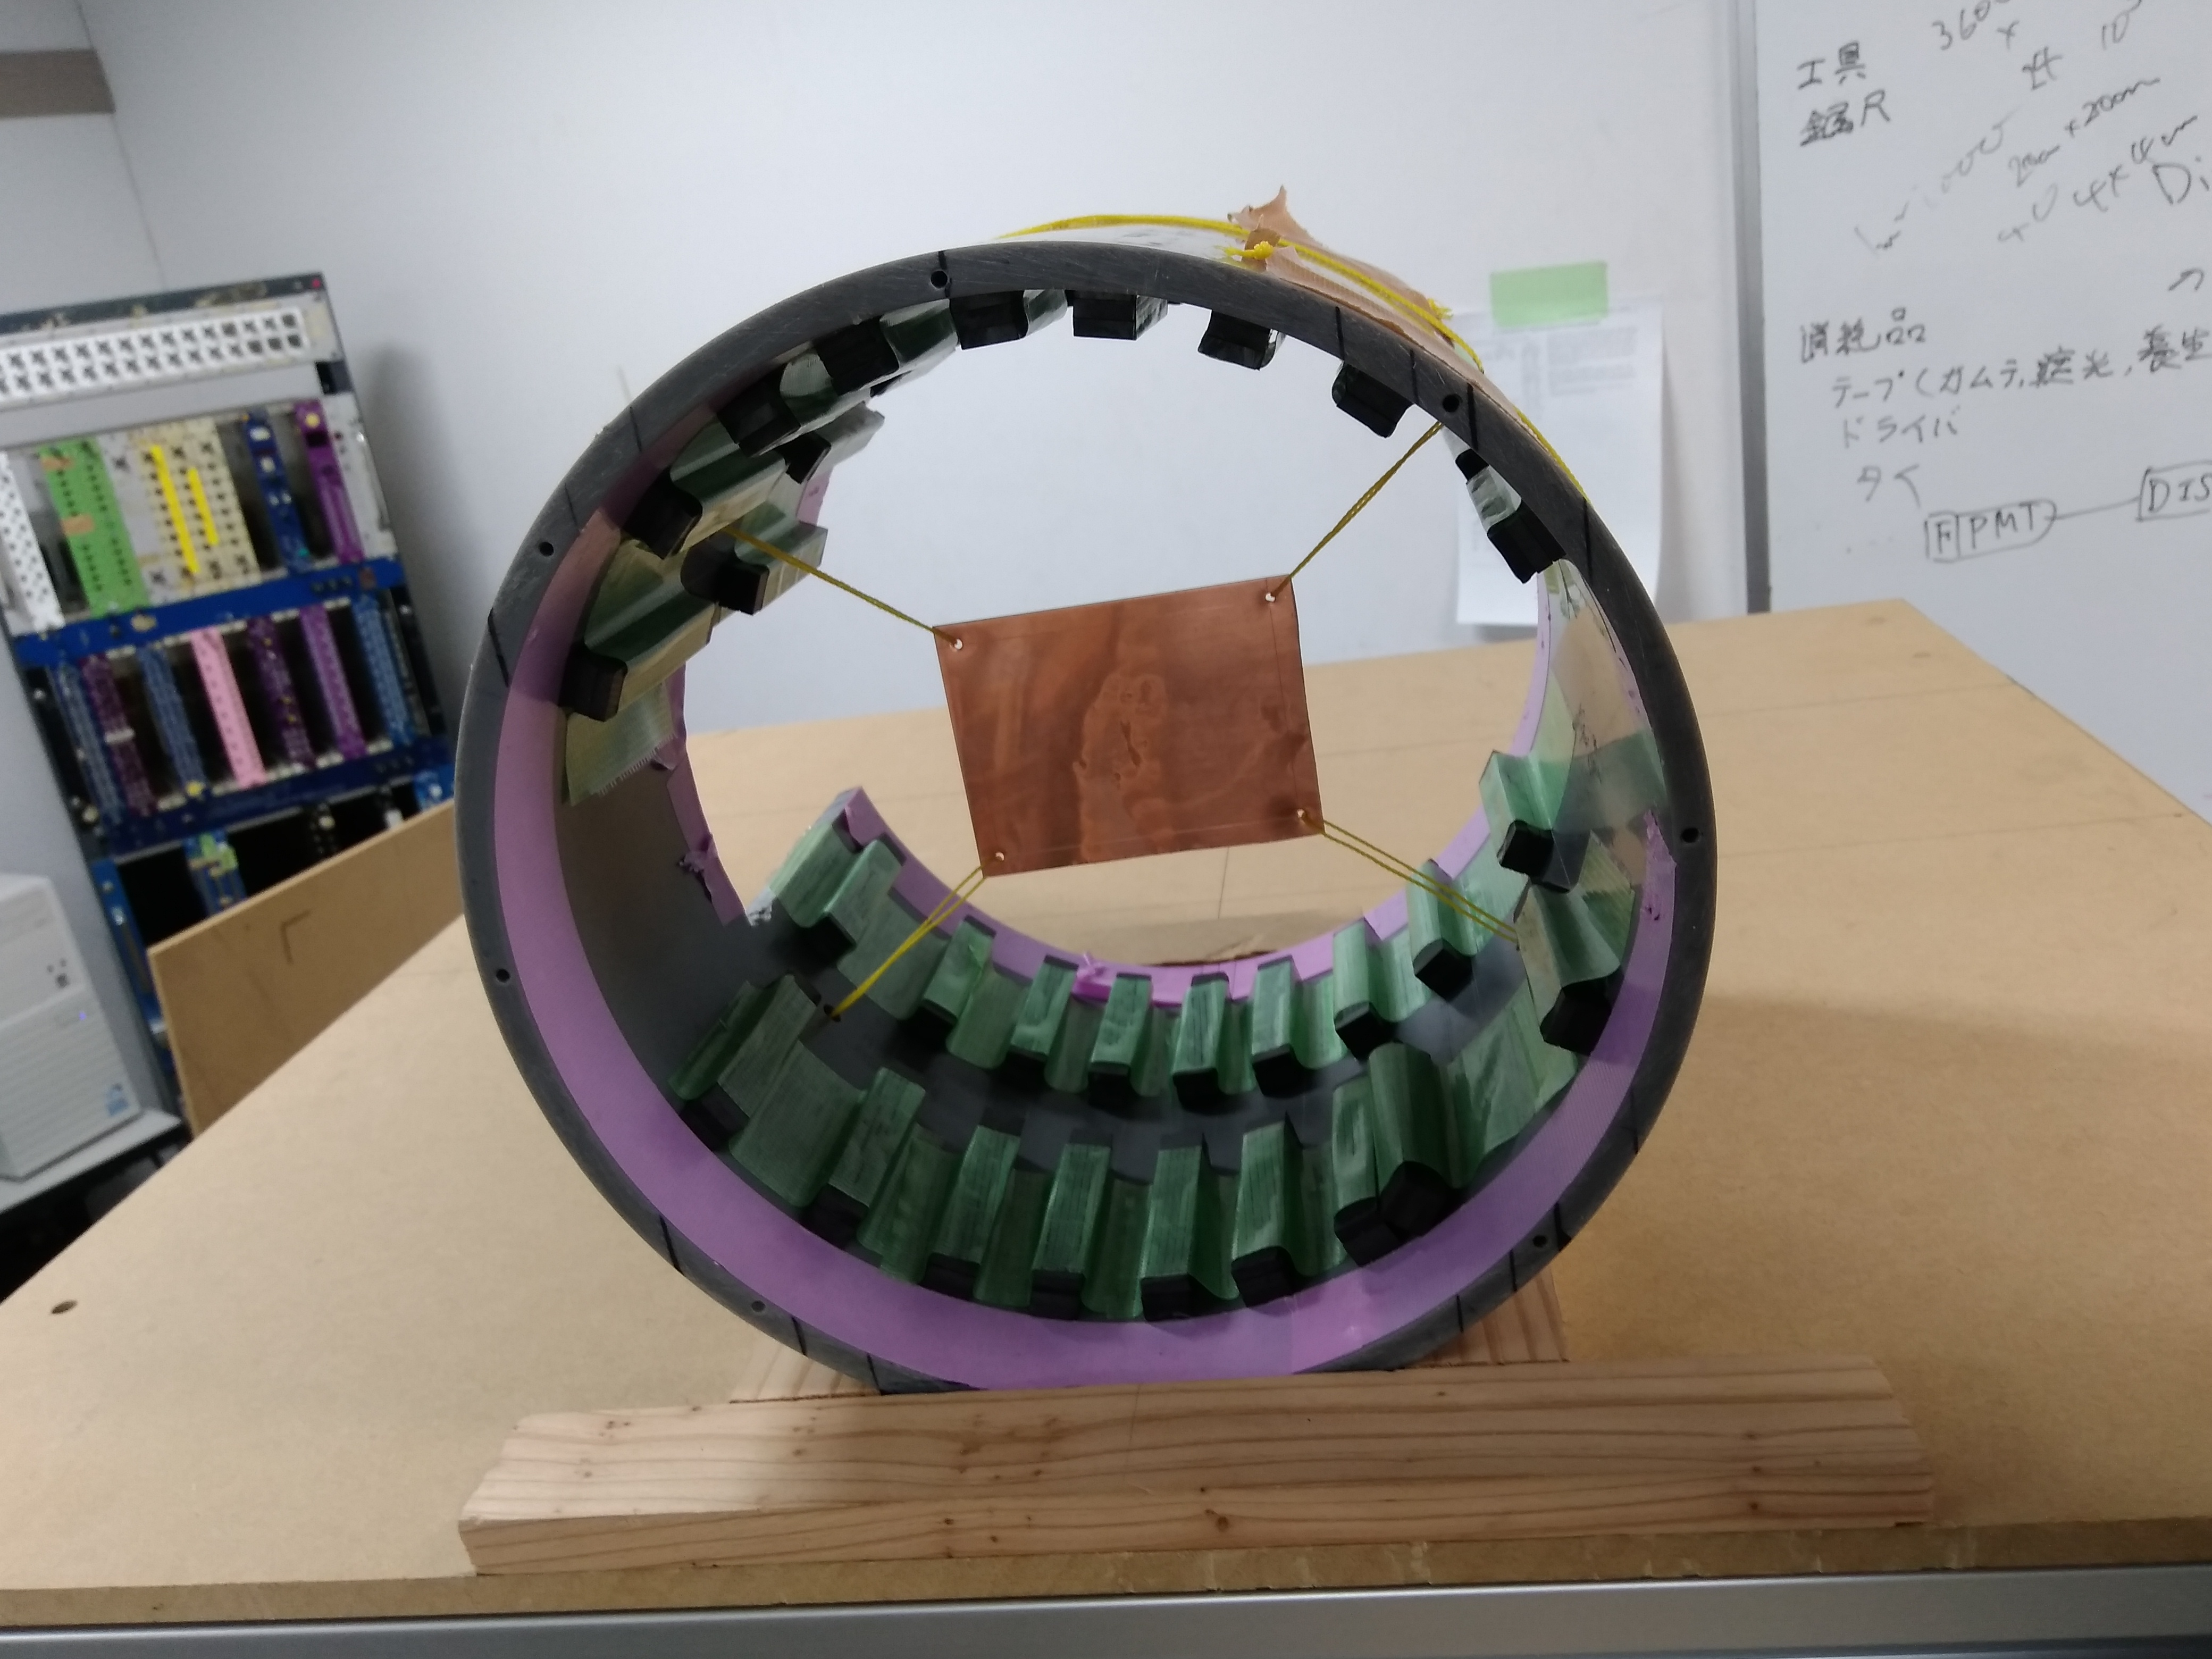
\includegraphics[width=1\textwidth]{figure/tajima/mag.jpg}
      \caption{磁場発生装置と標的 \protect\footnotemark}
      \label{tar_mag}
    \end{center}
  \end{minipage}
\end{figure}
\footnotetext{写真では下方の磁石が外れているが,これは実験前に修復した.}

\subsubsection{磁石の発生原理について: $\cos \theta$配置}
磁場装置は$\cos n\theta$巻き($n=1$)の電磁石を参考に作成した.
$\cos n \theta$巻きの電磁石の考え方は以下のものである.
下図\ref{cos2},\ref{cos4}のように,十分長い円環上を電流が$z$軸方向に流れているとする.
そして電流密度が$\cos n\theta$(ここで$\theta$は円柱座標($r,\theta,z$)における$\theta$で,$n$は整数)に比例したとする.
すると原点付近の領域に, $2n$極磁場が形成されるというものである.
導出の概略は,円環各点が形成する磁場をその点の周りでテーラー展開し,これを$\theta$について角度積分することで$2n$極磁場を形成する項のみが残るというものである.

\begin{figure}[H]
  \begin{minipage}{0.45\hsize}
    \begin{center}
      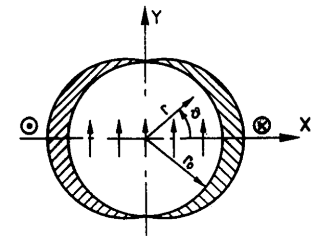
\includegraphics[width=0.8\textwidth]{figure/tajima/cos.png}
    \end{center}
    \caption{$\cos\theta$ : 2極磁石}
    \label{cos2}
  \end{minipage}
  \hfill
  \begin{minipage}{0.45\hsize}
    \begin{center}
      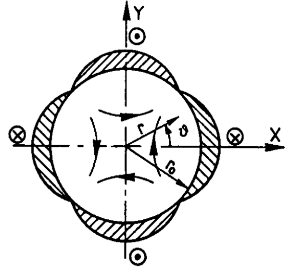
\includegraphics[width=0.7\textwidth]{figure/tajima/cos2.png}
    \end{center}
    \caption{$\cos2\theta$ : 4極磁石}
    \label{cos4}
  \end{minipage}
\end{figure}
%\renewcommand{\thefootnote}{\fnsymbol{footnote}}
\footnotetext{上図はKEKホームページ「加速器用超電導磁石(OHO11ogitsu20110906.pdf)」より引用}%画像引用は参考文献にしなくてよい?

作成の手軽さから,磁場発生源には電磁石ではなく永久磁石(セラミック磁石)を用いた.
電磁石における電流密度を,永久磁石の分布密度で置き換え,
磁石の分布密度が$|\sin\theta|$に比例するようにした.
$\sin\theta$としたのは磁石の向きをすべて動径方向に向けると,電磁石に比べ磁場の方向が$\pi/2$だけずれるためである.
また磁石の磁場方向は$0<\theta<\pi$と$\pi<\theta<2\pi$で動径方向に対して正と負になるようにした.
作成に入る前に考えた配置をFEMMを用いてシミュレートし,磁場の一様性を確認した.


実際に有限の長さの磁石で磁場装置を作成するにあたって,図\ref{tar_mag}のように磁石を長手方向に間隔を開けて二巻き配置した.
(一巻あたり磁石の数は18個である.)
長手方向の間隔は$30(\mathrm{mm})$で,間隔を開けることにより長手方向に隙間を空けずに磁石を詰めたときに比べて,
磁力線が緩和され長手方向に磁場の一様性が増すと考えたためである.

\newpage
\subsection{予備実験}
%\subsubsection{プラスチックシンチレータの宇宙線較正}

\subsubsection{NaIのゲイン測定}
本実験で用いるNaI検出器が出力する信号は,NaIの9本とフィンガーカウンターの計10個であった.
一方でNaIの信号の処理に用いるWFDの入力できるチャンネル数は8つであった.
このため,WFDに入力する前にNaIからの信号をアナログで足し合わせて信号の数を絞る必要があった.
NaI結晶自体の差から発光量も違い,NaIに付属するPMTのゲインはHVに対する依存性が個体毎に大きく異なる.
一方で,足し合わせるNaIの信号は同じエネルギーに対して同じにしなければならかったためそれぞれのNaIのゲインの測定を行った.
この測定したゲインからどうのようにNaIからの信号を足し合わせるかを決めた.

NaIのゲイン測定するためにHV値を変えながら線源$^{137}\mathrm{Cs}$を用いて,検出器用に用意した計11本のNaI(1から順番に番号を付けた)の電荷を測定を行った.
この線源は661.7keVのガンマ線を放出する.\cite{IAEA_ENSDF}
そのため,これを光電ピークと考えられるところでそれぞれガウシアンでFittingし,得られた平均値をゲインとした.
さらにゲインについて以下の式が成り立つとし,両対数でFittingを行った.\cite{Hamamatsu_PMT}
\begin{equation}
\mathrm{Gain}(\mathrm{pC})=a*\mathrm{HV}(\mathrm{kV})^b  
\end{equation}
ただし$a, b$はFitting パラメータである.
その結果を図にしたものが図\ref{GainHV}で,
縦軸をゲインにあたる電荷$(\mathrm{pC})$,横軸をHV値$(\mathrm{kV})$とした.
また各HVでのエネルギー分解能とHVの関係をあらわした図が図\ref{HVreso}で,
縦軸を分解能,横軸をゲイン$(\mathrm{pC})$とした.
ただし分解能はガウシアンの$\sigma$を電荷で割ったものある.
\begin{figure}[H]
  \begin{minipage}{0.45\hsize}
    \begin{center}\hspace*{-1em}
      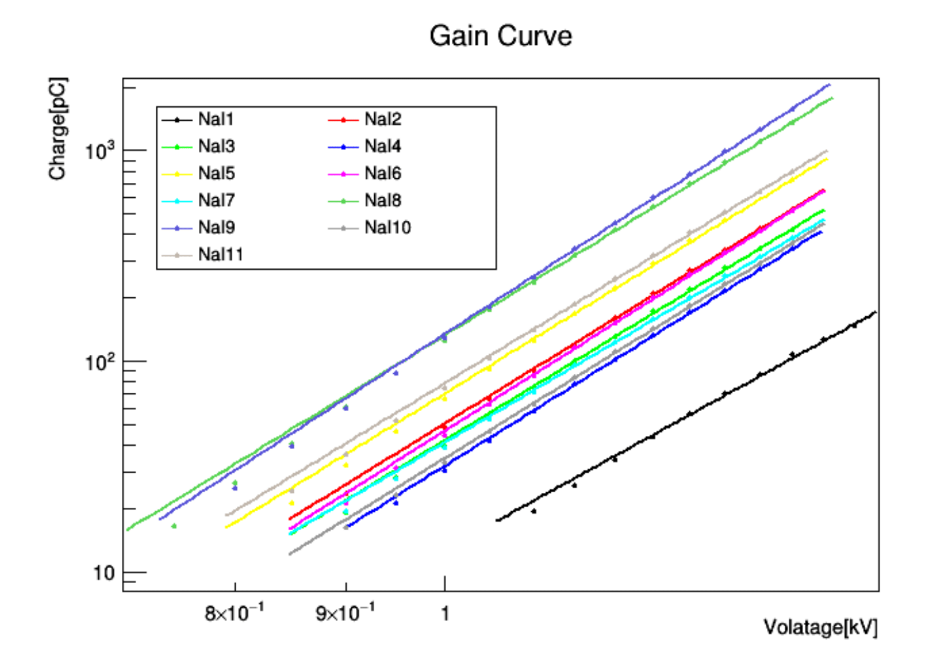
\includegraphics[width=1.1\textwidth]{figure/tajima/gain_curve.png}
    \end{center}
    \caption{ゲインとHVの対応}
    \label{GainHV}
  \end{minipage}
  \hfill
  \begin{minipage}{0.45\hsize}
    \begin{center}
      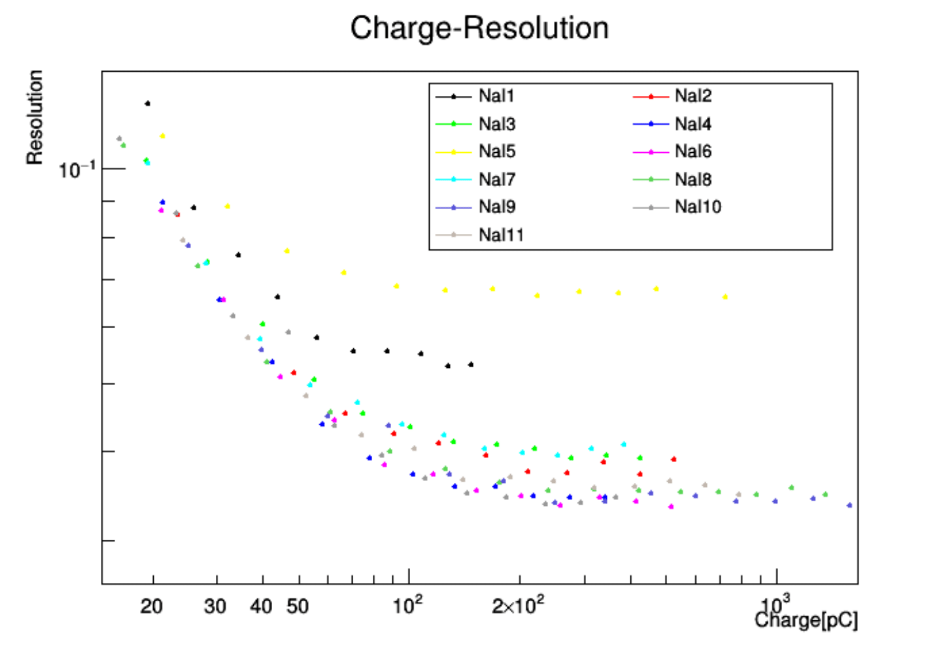
\includegraphics[width=1.1\textwidth]{figure/tajima/charge_resolution.png}
    \end{center}
    \caption{ゲインと分解能の対応}
    \label{resoHV}
  \end{minipage}
\end{figure}
この結果, NaI1はゲインが低く,NaI5に関しては分解能が低かったため,本実験では用いないことにした.
(以降,NaI1,5で測定を行わないことにした.)
またNaI10は分解能が良かったため,足し合わせず真ん中に配置するNaIとした.

今回測定に用いた線源のエネルギー661.7keVに対して,実際の測定では最大50MeV程度のエネルギーを測定することになる.
そのため,高いエネルギー領域においても上のゲイン曲線が成り立っていることの確認を行った.
崩壊電子の最大エネルギーが約$\sim 50[\mathrm{MeV}]$であり,WFDの上限の半分$1[\mathrm{V}]$($500[\mathrm{pC}$])になるように設定した.%電圧と電荷の対応関係について要説明
このゲインを揃えたHVの設定で宇宙線を測定した.
そして,得られた電荷分布をLandau関数をガウシアンで畳み込み積分した関数(以下,Langau関数とよぶ)で
Fittingをした.
このLangau関数の最頻値をゲインとすると,表\ref{nai_gain}のようになった.
このゲインの値が近く,また分解能の近いものを足し合わせるペアとし,
これを(2,7),(3,9),(4,6),(8,11)の4組に決めた.
これらのペアのずれはいずれも$10\%$未満となった.% なにがかを明記


\begin{table}[H]
  \begin{minipage}[t]{0.45\textwidth}
    \begin{center}
    \caption{宇宙線の測定結果}\label{nai_gain}
      \begin{tabular}{|c|c|}\hline
        NaI No. & Gain[pC]\\ \hline \hline
        2 & 2530 \\ \hline
        3 &2387 \\ \hline
        4 &2352 \\ \hline
        6 &2397 \\ \hline
        7  &2579 \\ \hline
        8  &2423 \\ \hline
        9  &2164 \\ \hline
        11  &2393 \\ \hline
      \end{tabular}
    \end{center}
  \end{minipage}
  \hfill
  \begin{minipage}[t]{0.45\textwidth}
    \begin{center}
    \caption{NaIのHV設定}\label{HV}
      \begin{tabular}{|c|c|}\hline
      NaI No.&HV[V]\\ \hline \hline
      % 1 & 1342 \\ \hline
      2 & 1050 \\ \hline
      3 & 1082 \\ \hline
      4 & 1125 \\ \hline
      % 5 & 1002 \\ \hline
      6 & 1062 \\ \hline
      7 & 1089 \\ \hline
      8 & 913 \\ \hline
      9 & 913 \\ \hline
      10 & 1112 \\ \hline
      11 & 984 \\ \hline
      \end{tabular}
    \end{center}
  \end{minipage}
\end{table}

さらに本実験におけるNaIの配置を表\ref{haichi}になるように決めた.
配置を決めるにあたって,以下の事柄を考慮した.
\begin{itemize}
\item エネルギー重心を求める観点からペアを中心から等距離になるように配置
\item 角でのGainが不足しないように, Gainの高いペアを角に配置%要説明
\item 本番セットアップでの宇宙線較正を想定して,上下にペアがこないように配置%要説明
\end{itemize}
\begin{table}[H]
  \begin{center}
    \caption{ビーム正面からみたNaIの配置図}\label{haichi}
    \begin{tabular}{|c|c|c|}\hline 
      \cellcolor{yellow}3&\cellcolor{red}2&\cellcolor{yellow}9\\ \hline
      \cellcolor{cyan}4&10&\cellcolor{red}7\\ \hline
      \cellcolor{green}8&\cellcolor{cyan}6&\cellcolor{green}11\\ \hline
    \end{tabular}
  \end{center}
\end{table}
\newpage
\subsubsection{NaIの宇宙線較正}
NaIでエネルギーを測定するために, 宇宙線で較正を行った.
先にもとめたHV値のもとで,それぞれのNaIで宇宙線を測定した.%要実験セットアップ詳細
得られた電荷分布を,Langau関数でFittingをした.(図\ref{langau})
そして得られた最頻値を宇宙線が落としたエネルギーとした.% ??

次にGeant4を用いて,天頂角分布で宇宙線モンテカルロシミュレーションを行った.
図\ref{MC2}はシミュレーションによるエネルギー分布で,縦軸にカウント数,横軸にエネルギーを$24\mathrm{MeV}$で規格化したものをとった.
このエネルギー分布にLandau関数でFittingし,%してない
得られた最頻値と測定によって得られた最頻値でエネルギー較正を行った.

\begin{figure}[H]
  \begin{minipage}{0.45\hsize}
    \begin{center}\hspace*{-1em}
  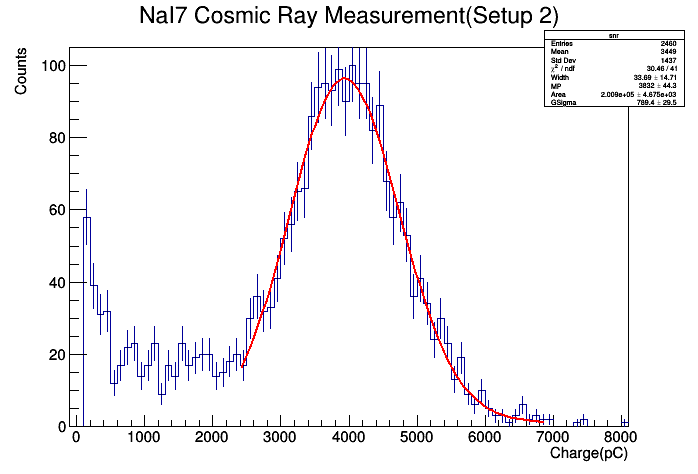
\includegraphics[width=1\textwidth]{figure/tajima/NaI7_Setup2.png}
      \caption{測定データのLangau Fitting}\label{langau}
    \end{center}
  \end{minipage}\hfill
  \begin{minipage}{0.45\hsize}
    \begin{center}
      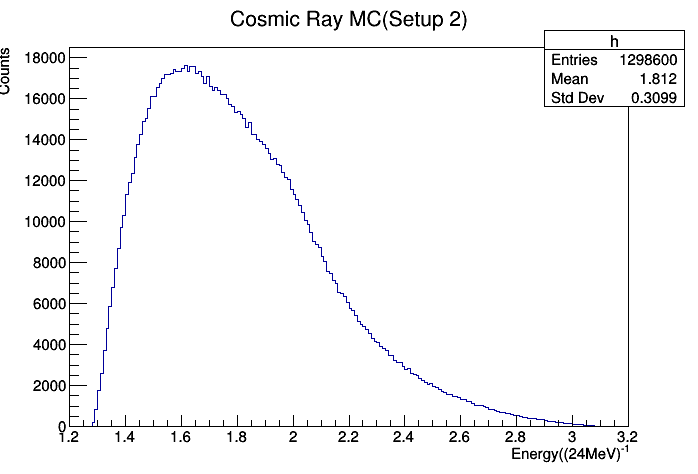
\includegraphics[width=1\textwidth]{figure/tajima/MC2.png}
      \caption{c}\label{MC2}
    \end{center}
  \end{minipage}
\end{figure}

図\ref{cali}は宇宙線較正の結果を図にしたもので,
縦軸をFADCで測定された電荷$(\mathrm{pC})$,横軸をエネルギー$(\mathrm{MeV})$としたものである.
\begin{figure}[H]
  \centering
      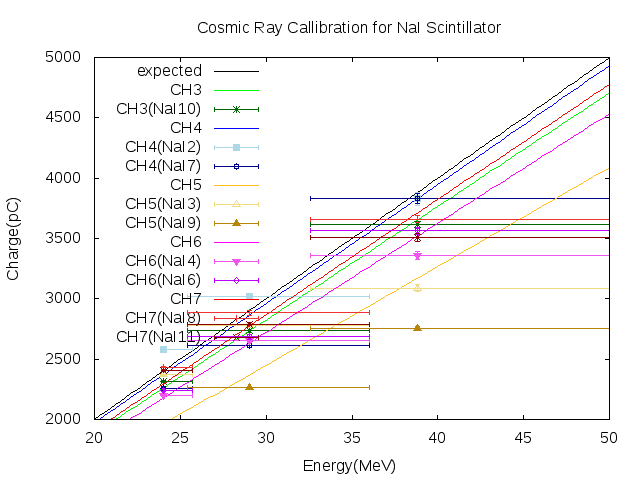
\includegraphics[width=0.7\textwidth]{figure/tajima/fit.png}
      \caption{宇宙線測定の電荷とエネルギーの対応関係}\label{cali}
\end{figure}
\newpage
\subsubsection{磁場測定}
磁場装置の測定を行った.
3軸テスラメータで銅板を置く範囲を,$1\mathrm{cm}$間隔で計63点を測定した.
本実験の測定中に磁石が外れてしまったので,磁石が外れる前後のデータとして実験前と実験後に測定した.

測定した結果を以下の表\ref{MF1},\ref{MF2}に記す.
$x,y$の単位は$(\mathrm{mm})$で,磁場の単位は$(\mathrm{G})$である.
原点を銅板の中心とし, $y,z$軸を鉛直方向上向きとビーム方向にとった.
\begin{table}[H]
  \begin{center}
    \caption{各点の磁場の強さ(磁石が外れる前)}\label{MF1}
    \begin{tabular}{|c||c|c|c|c|c|c|c|c|c|}\hline
       y\textbackslash x & -4 & -3 & -2 & -1 & 0 & 1 & 2 & 3 & 4 \\ \hline \hline
      3 & 51.48 & 54.98 & 55.33 & 55.55 & 55.42 & 54.77 & 54.44 & 53.27 & 51.75 \\ \hline
      2 & 56.25 & 56.78 & 56.87 & 56.84 & 56.41 & 56.16 & 55.93 & 55.71 & 55.35 \\ \hline
      1 & 57.15 & 57.50 & 57.39 & 57.11 & 56.72 & 56.53 & 56.48 & 56.50 & 56.44 \\ \hline
      0 & 57.60 & 57.49 & 57.19 & 56.72 & 56.54 & 56.48 & 56.53 & 56.58 & 55.98 \\ \hline
      -1 & 56.66 & 56.78 & 56.66 & 56.48 & 56.39 & 56.34 & 56.35 & 56.31 & 56.12 \\ \hline
      -2 & 53.45 & 54.74 & 55.29 & 55.54 & 55.60 & 55.60 & 55.53 & 55.14 & 54.3 \\ \hline
      -3 & 50.62 & 51.95 & 53.45 & 53.93 & 54.20 & 54.20 & 54.05 & 53.11 & 51.25 \\ \hline
    \end{tabular}
  \end{center}
\end{table}
\begin{table}[H]
  \begin{center}
    \caption{各点の磁場の強さ(磁石が外れた後)}\label{MF2}
    \begin{tabular}{|c||c|c|c|c|c|c|c|c|c|}\hline
       y\textbackslash x & -4 & -3 & -2 & -1 & 0 & 1 & 2 & 3 & 4 \\ \hline \hline
      3 & 55.41 & 55.93 & 55.79 & 54.78 & 53.30 & 50.73 & 46.89 & 46.34 & 41.95 \\ \hline
      2 & 57.25 & 57.06 & 56.28 & 54.92 & 53.77 & 52.01 & 49.83 & 48.45 & 48.44 \\ \hline
      1 & 57.72 & 57.30 & 56.52 & 55.61 & 54.34 & 52.97 & 51.84 & 51.08 & 50.49 \\ \hline
      0 & 57.55 & 56.94 & 56.30 & 55.54 & 54.61 & 53.67 & 52.98 & 52.40 & 52.34 \\ \hline
      -1 & 57.00 & 56.57 & 55.94 & 55.24 & 54.58 & 53.99 & 53.45 & 53.05 & 52.73 \\ \hline
      -2 & 55.48 & 55.37 & 55.04 & 54.64 & 54.30 & 53.83 & 53.39 & 52.53 & 51.81 \\ \hline
      -3 & 52.23 & 53.03 & 53.28 & 53.29 & 53.18 & 52.71 & 52.00 & 51.51 & 50.12 \\ \hline
 \end{tabular}
  \end{center}
\end{table}
$g$因子の計算に用いる磁場を得るために,予め頂いたビームプロファイルのデータ($\sigma_x=33.3037(\mathrm{mm}),\ \sigma_y=19.6668(\mathrm{mm})$)を用いて
加重平均をとった.
結果,磁石が外れる前後の磁場がそれぞれ$56.06\pm 1.20\  (\mathrm{G})$ と$53.97\pm 2.36\  (\mathrm{G})$ と求まった.
\newpage
\subsection{ビームを用いた本実験}
\subsubsection{タイムスケジュール}
本実験におけるタイムスケジュールは以下の通りである.
\begin{itemize}
\item 2/25 (Sun.)\\
  13:00   東海村到着,前日準備
\item 2/26 (Mon.) $\sim$ 2/27 (Tue.)\\
  9:00 $\sim$ロシアグループの傍らで寿命を測定, セットアップの確認
\item 2/28 (Wed.)\\
  12:30   ロシアグループの実験終了,\ P2ターゲットで実験開始\\ % P2ターゲットとは??
  12:30 - 21:30 セットアップの確認\\
  21:47 - 24:00 磁場ターゲットを置いて,\ $g$因子をNaIのみで測定\\
  24:20 - 29:50 磁場ターゲットを置いて,\ $g$因子をPSを加えて測定(測定の途中で磁石が外れる)%磁場の測定タイミングも記載したい
\item 3/1 (Thu.)\\
  7:20 - 8:10 銅板標的を置いて, エネルギーと寿命を測定\\%標的とターゲットの表記ゆれ
  8:30   ビームストップ\\%ビームストップの意味がおそらく伝わりにくい?下流のミューオンラインとの区別
  8:30 - 14:30 放射線チェック, 片付け \\%放射線チェックでは実験用になにかを測定シタように勘違いするかも?
  14:30 $\sim$ 帰宅
\end{itemize}
\subsubsection{セットアップ}
%本実験の寿命測定におけるセットアップを図\ref{set_lifetime}に記す.
%\begin{figure}[H]
%  \centering
%  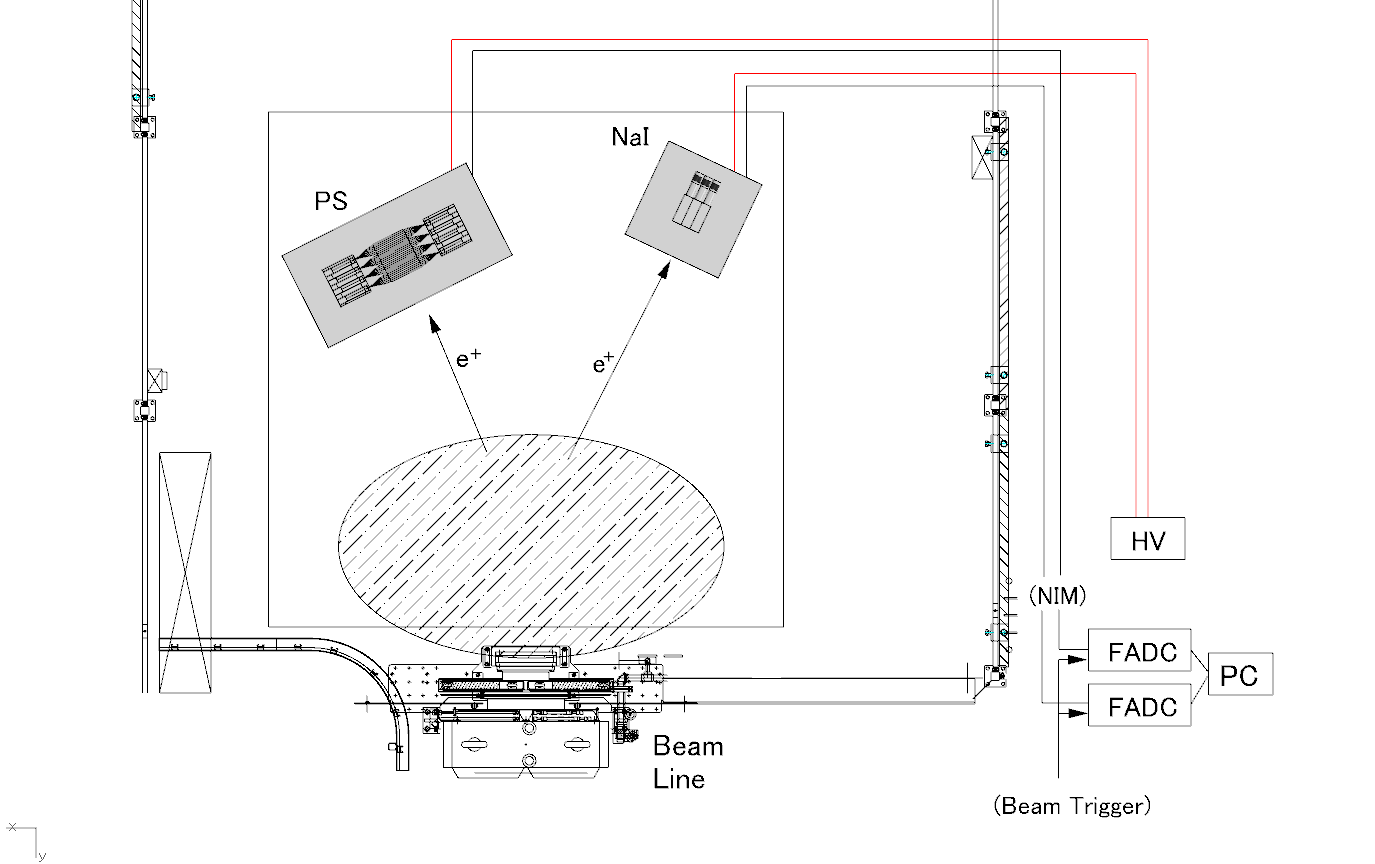
\includegraphics[width=0.7\textwidth]{figure/tajima/lifetime.png}
%  \caption{寿命測定のセットアップ}
%  \label{set_lifetime}
%\end{figure}
この節では本実験のセットアップについて記す.\\
まず寿命測定のセットアップについて図\ref{set_life},\ref{set_life2}に記す.
図\ref{set_life}が上空からみたセットアップ図で,図\ref{set_life2}が実際のセットアップの写真である.
ここでFC, PSはフィンガーカウンターとプラスチックシンチレータの略で, Targetには先に述べた銅板標的を用いた.
今回の検出器では解析の都合から,陽電子がNaIでは1パルスあたり5,6個にプラスチックシンチレータでは%個になるように調整を行った.
具体的にはターゲットから測定器までの距離をビーム$1(\mathrm{pulse})$あたりの陽電子のカウント数から決めた.
\begin{figure}[H]
  \begin{minipage}{0.45\hsize}
    \begin{center}
      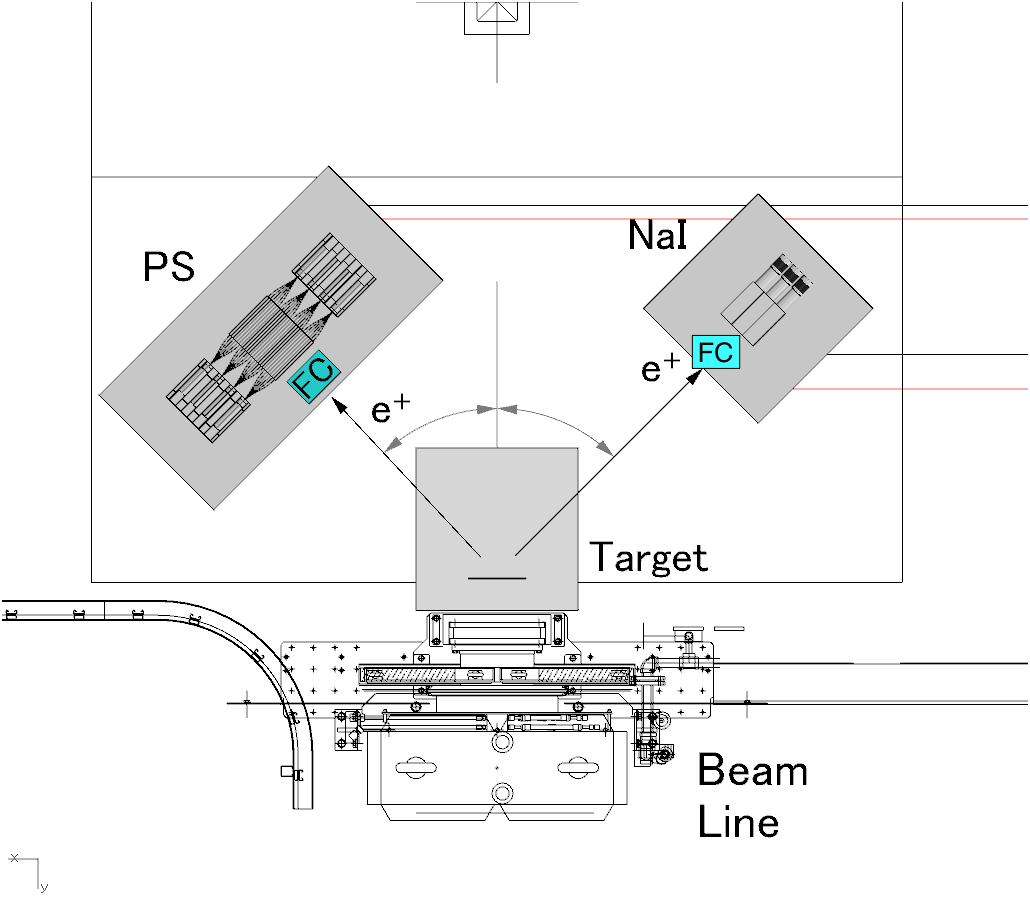
\includegraphics[width=1\textwidth]{figure/tajima/set_lifetime.png}
      \caption{寿命測定のセットアップ図}
      \label{set_life}
    \end{center}
  \end{minipage}
  \begin{minipage}{0.45\hsize}
    \begin{center}
      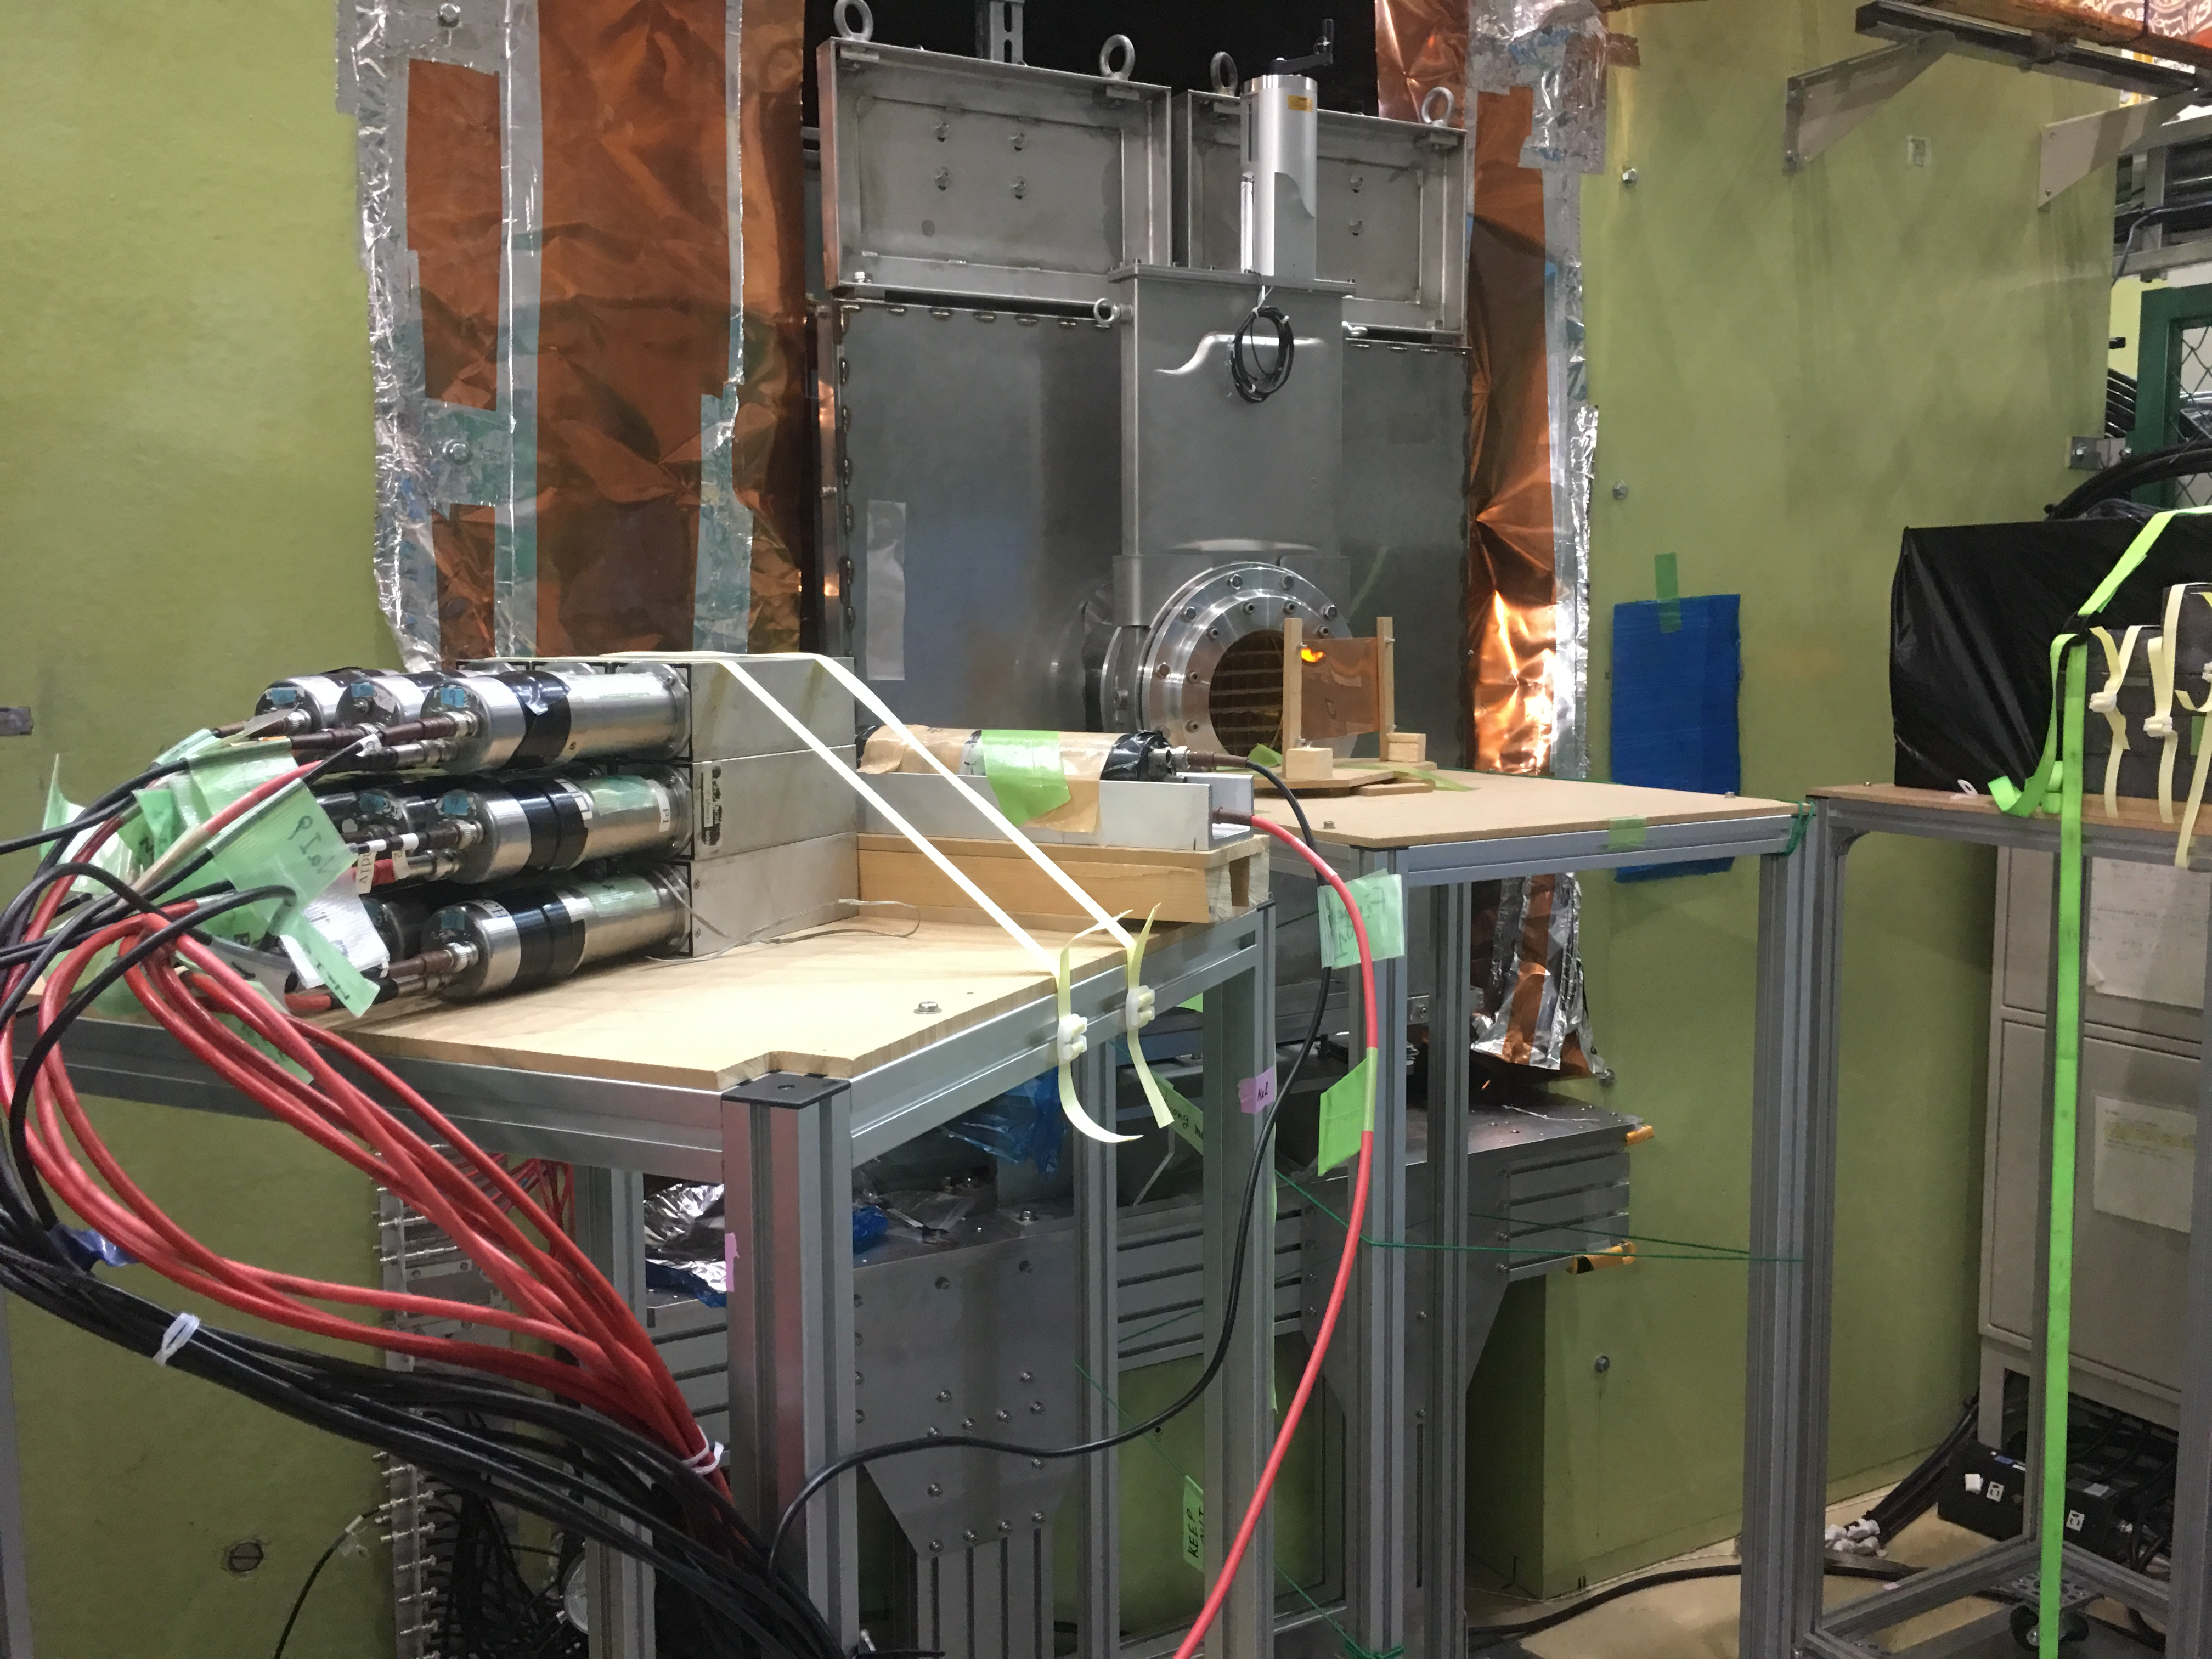
\includegraphics[width=1\textwidth]{figure/tajima/set_lifetime_1.png}
      \caption{寿命測定のセットアップ(写真)}
      \label{set_life2}
    \end{center}
  \end{minipage}
\end{figure}

次にエネルギー, $g$因子測定のセットアップについて図\ref{set_g_1}.\ref{set_g_2}に記す.
図\ref{set_life}が上空からみたセットアップ図で,図\ref{set_life2}が実際のセットアップの写真である.
ここでTargetには先に記した磁場印加標的を用いた.
寿命測定と同様に,ターゲットから測定器までの距離は,ビーム$1(\mathrm{pulse})$あたりの陽電子のカウント数から決めた.
\begin{figure}[H]
  \begin{minipage}{0.45\hsize}
    \begin{center}
      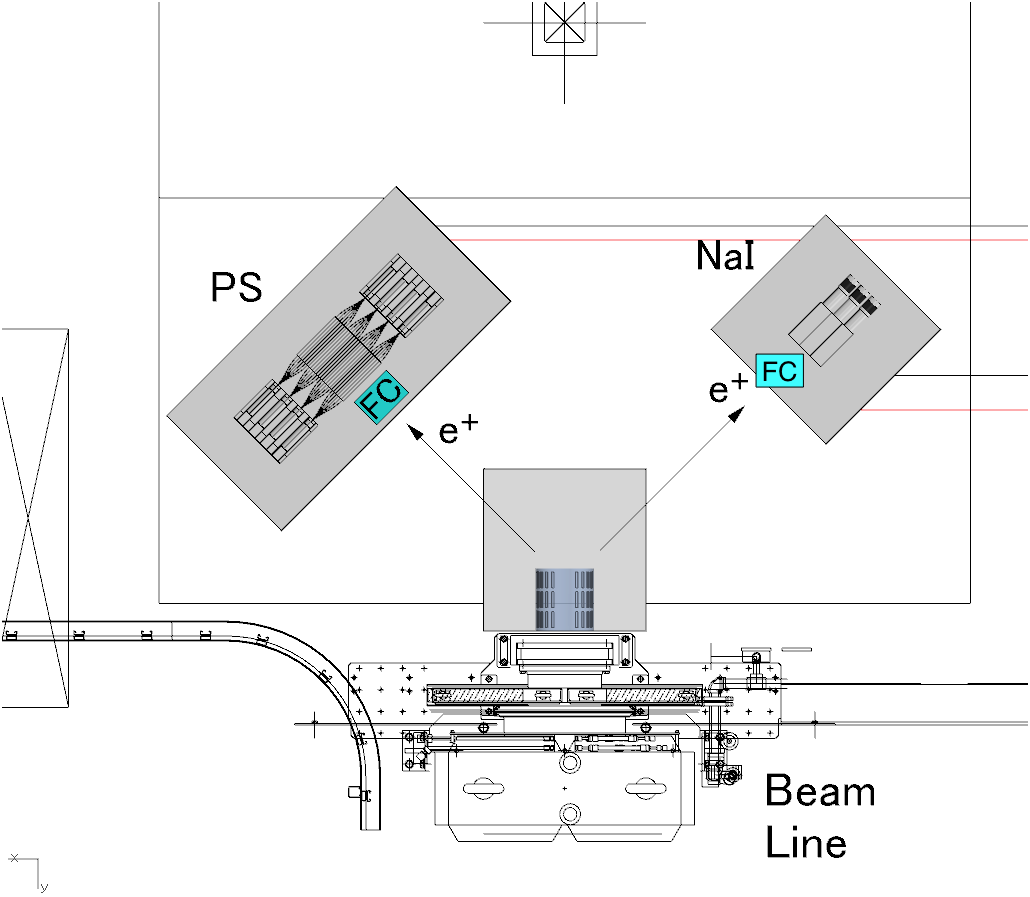
\includegraphics[width=1\textwidth]{figure/tajima/g-2_3.png}
      \caption{$g$因子測定のセットアップ}
      \label{set_g_1}
    \end{center}
  \end{minipage}
  \begin{minipage}{0.45\hsize}
    \begin{center}
      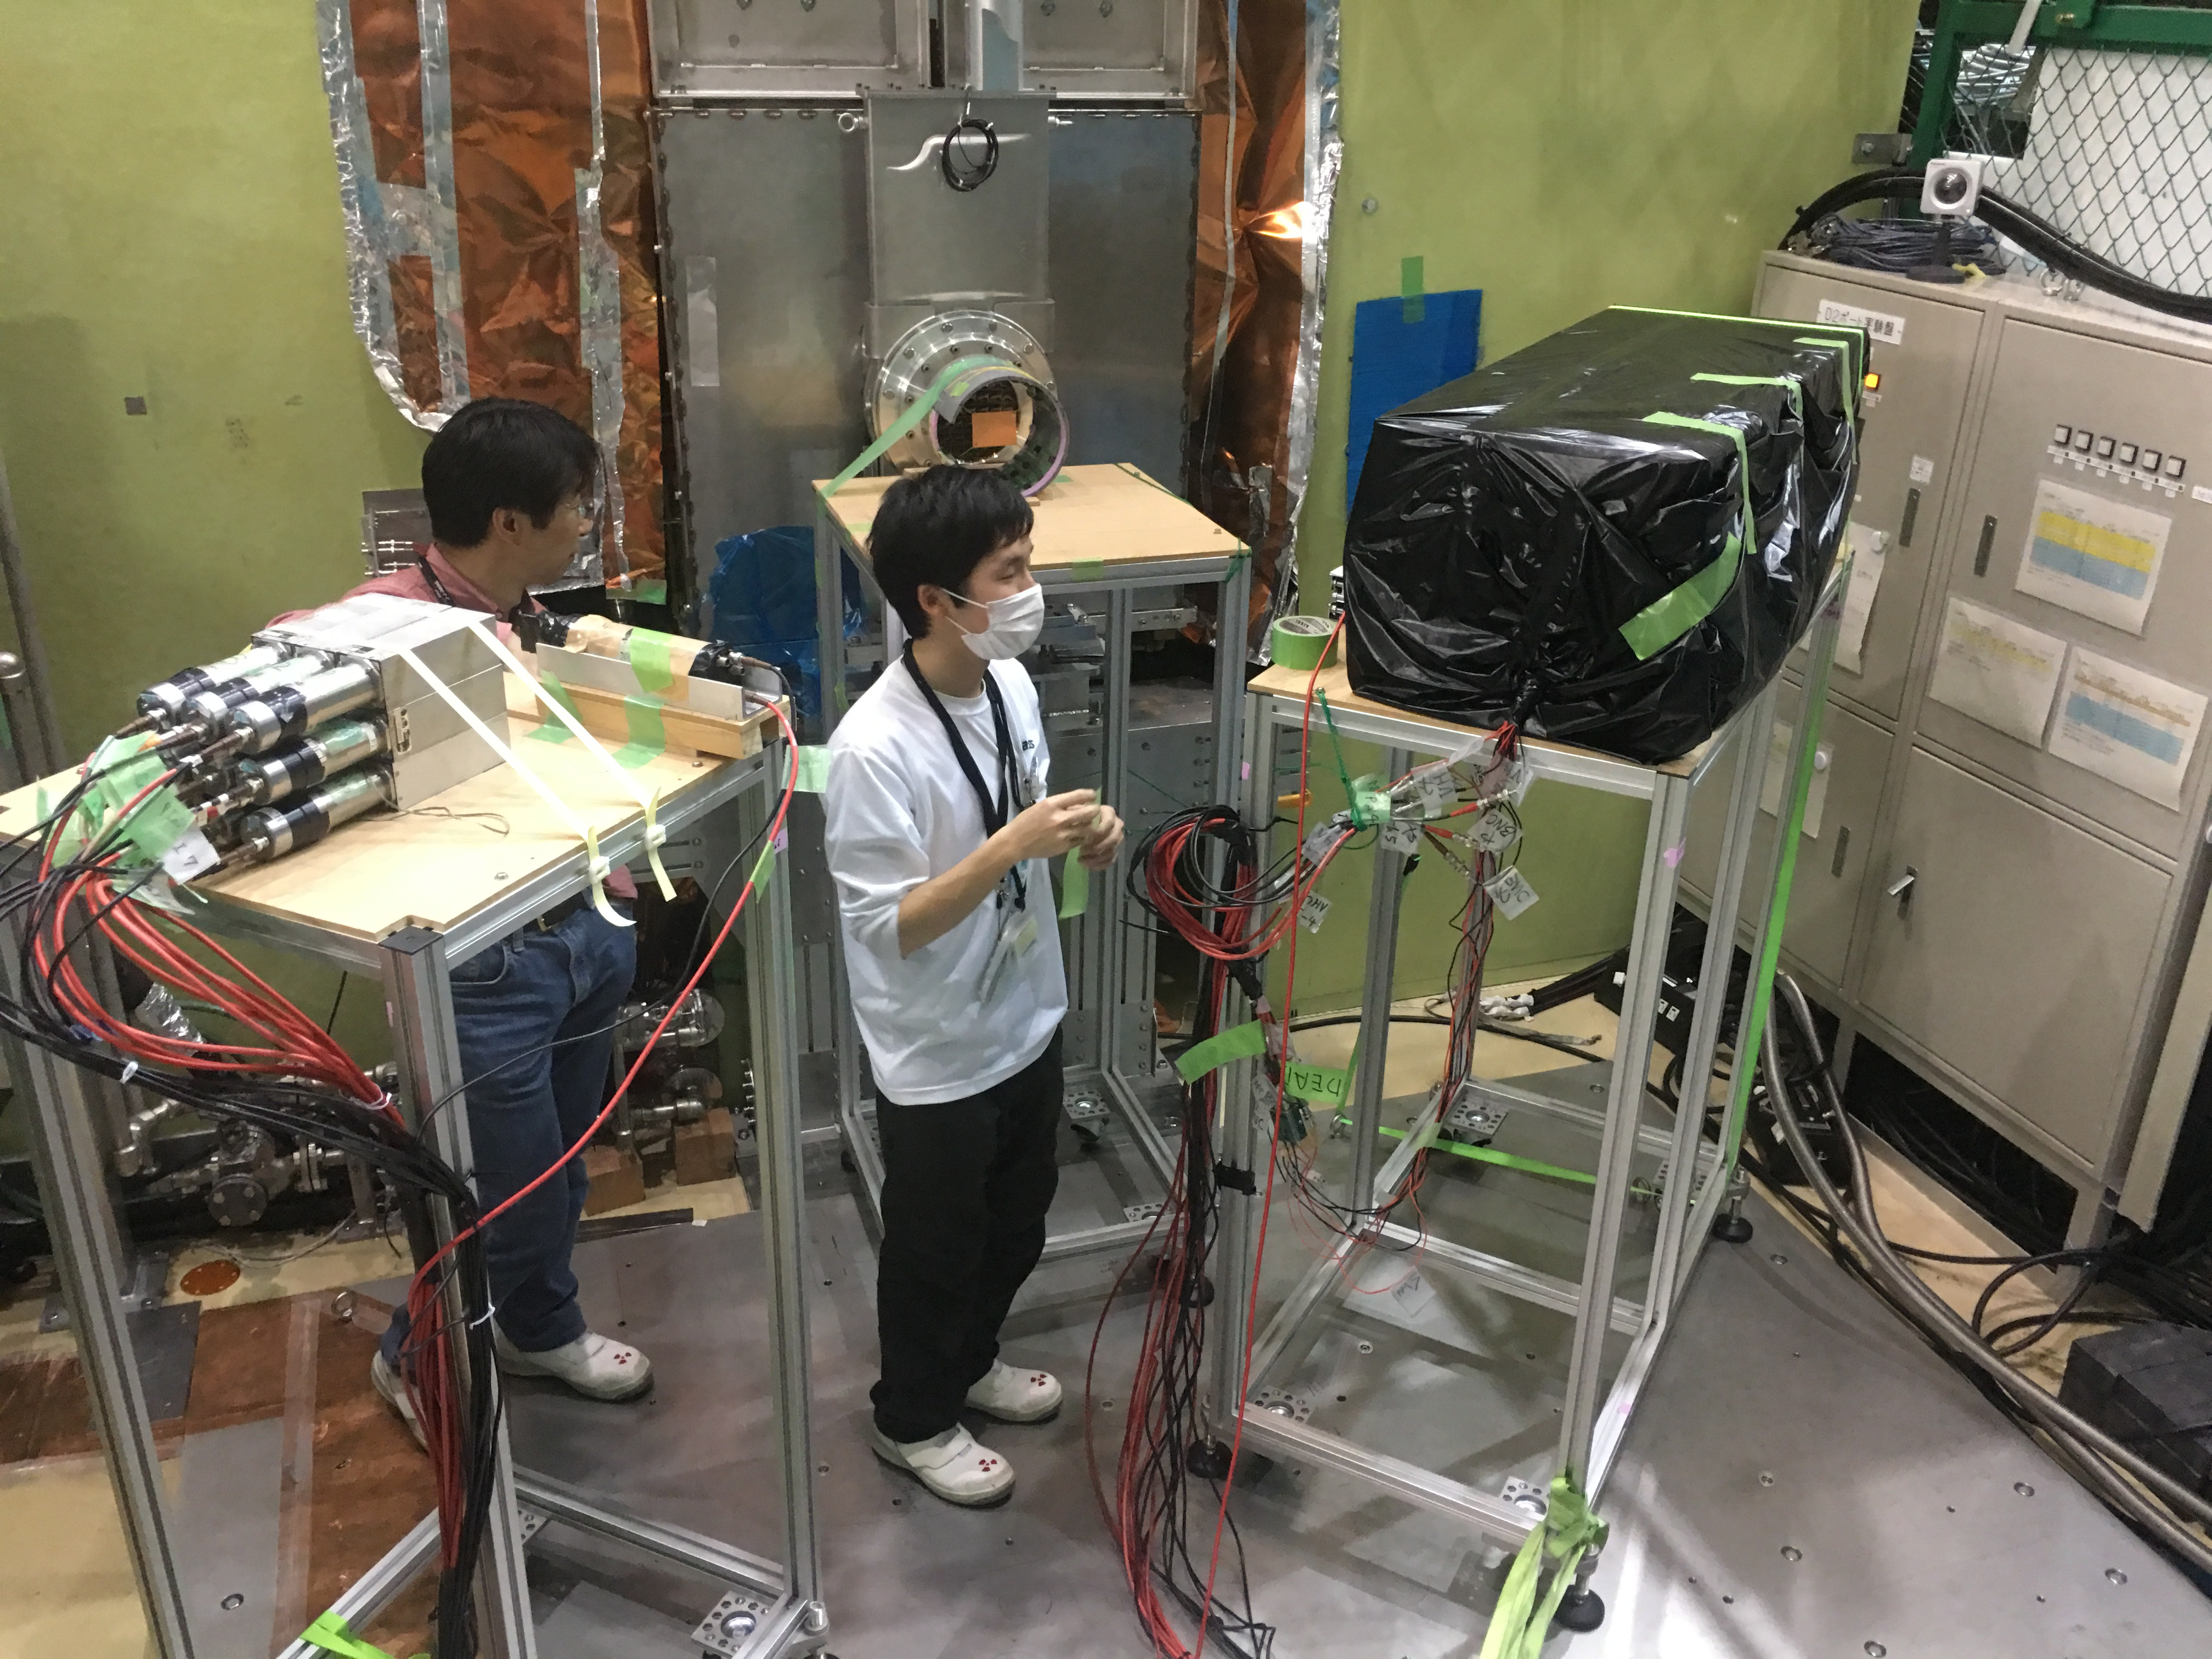
\includegraphics[width=1.1\textwidth]{figure/tajima/g.jpg}
      \caption{$g$因子測定のセットアップ(写真)}
      \label{set_g_2}
    \end{center}
  \end{minipage}
\end{figure}
\subsubsection{回路}
この節では本実験の回路について述べる.\\
図\ref{cir_PS},\ref{cir_nai}はNaI,プラスチックシンチレータの回路である.
ここでBeam TrigerはMLF施設からの信号で,WFDの外部Trigerとして接続した.
また図\ref{cir_PS}の$n-s$($n=1,2,3,4$, $s=a,b$)はプラスチックシンチレータの$n$層目のファイバーの片側から読み出される信号を意味する.
図中に記載している端子名(BNC, LEMO, MCX)は接続したケーブルの両端の端子名である.FADCはWaveform Digitizerの略である.
\begin{figure}[H]
  \begin{minipage}{0.45\hsize}
    \begin{center}
      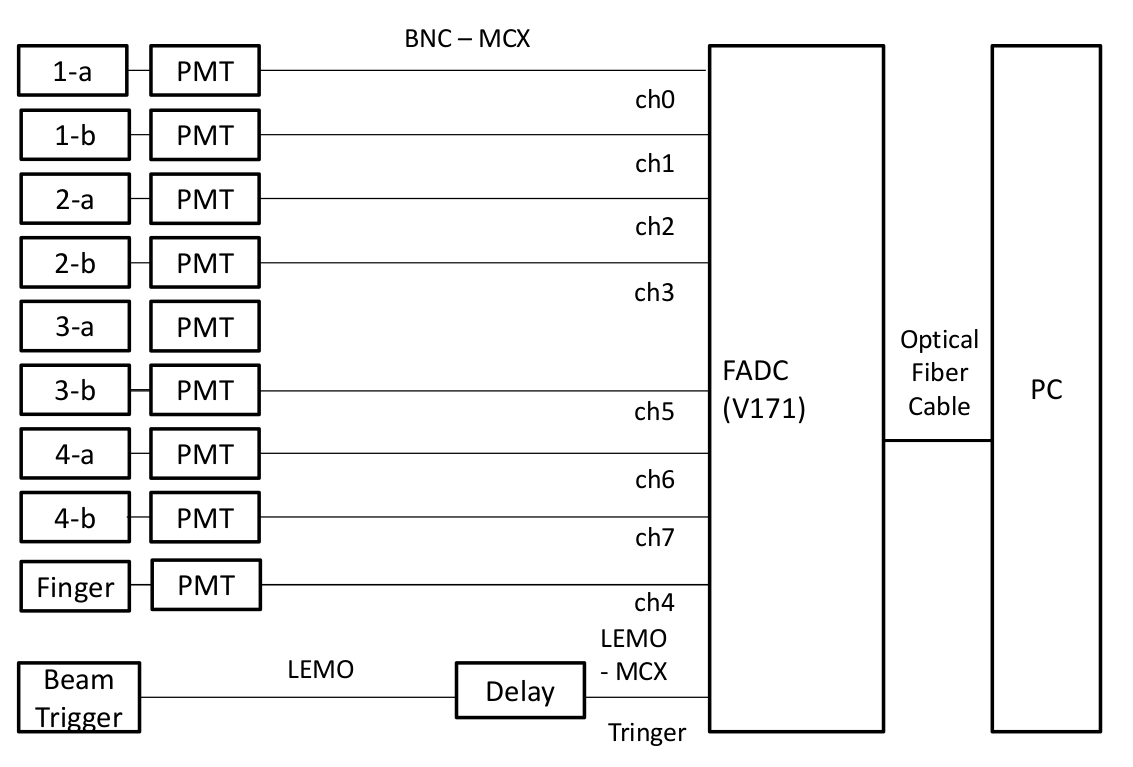
\includegraphics[width=1\textwidth]{figure/tajima/circuit_ps_2.png}
      \caption{プラスチックシンチレータ検出器用の回路}
      \label{cir_PS}
    \end{center}
  \end{minipage}
  \hfill
  \begin{minipage}{0.45\hsize}
    \begin{center}
      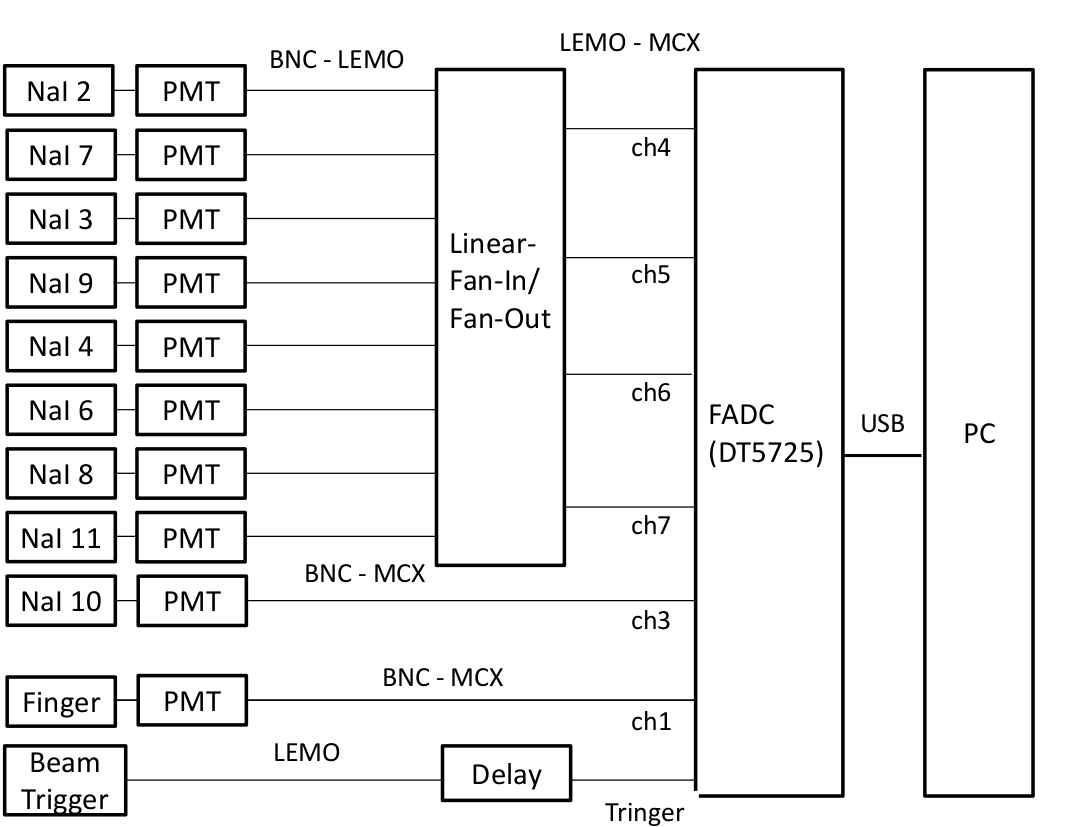
\includegraphics[width=1\textwidth]{figure/tajima/circuit_nai.png}
      \caption{NaI検出器用の回路}
      \label{cir_nai}
    \end{center}
  \end{minipage}
\end{figure}
本実験ではコリメータだけでは不十分で,
プラスチックシンチレータにおいても標的から飛んできた陽電子かどうかを判定するためのフィンガーカウンターを設置する必要性が浮上した.
そこでフィンガーカウンターを設置した.
その際にWFDの入力数が不足したため,中間でありデータの価値が低いであろうと考えたプラスチックシンチレータの3層目を片側読み出しにすることにした.

\subsubsection{実験手順}
本実験は以下の手順で行った.
\begin{enumerate}
  \item セットアップを調整した.
  \item ビームエリアの施錠を行い,ビームラインを開放した.%ビームエリアやビームラインの要説明
  \item ビームライン上のコリメーターを制御することで, \\ビーム1パルス当たりのレートを調整した.
    \\必要な場合はセットアップ調整からやり直した.
  \item データテイキングを開始した.
\end{enumerate}
%--------キリトリ線(下)--------
%\end{document}
